
\section{Testovanie}
\label{sec:testovanie}
Pre testovanie riešenia tejto práce sa využíva funkcia zodpovedná za evaluáciu modelov \textit{evaluate\_model} v scripte \textit{evaluation.py}
    podľa metrík ktoré boli spomenuté už vyššie.
Testovanie modelov prebieha ako určovanie presnosti týchto natrénovaných modelov.

\begin{figure}[H]
    \centering
    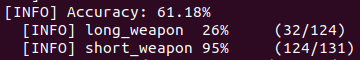
\includegraphics[width=0.75\textwidth]{testovanie}
    \caption{Príklad výstupu po testovaní modelu určujúceho typ zbrane.}
    \label{pic:testovanie}
\end{figure}

\begin{figure}[H]
    \centering
    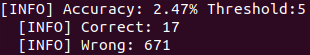
\includegraphics[width=0.7\textwidth]{testovanie_angle}
    \caption{Príklad výstupu po testovaní modelu určujúceho náklon zbrane.}
    \label{pic:testovanie}
\end{figure}
